% Preview source code

%% LyX 1.6.10 created this file.  For more info, see http://www.lyx.org/.
%% Do not edit unless you really know what you are doing.
\documentclass[parskip]{cs4rep}
\usepackage{graphicx}
\usepackage{listings}
\usepackage{color}

\definecolor{dkgreen}{rgb}{0,0.6,0}
\definecolor{gray}{rgb}{0.5,0.5,0.5}
\definecolor{mauve}{rgb}{0.58,0,0.82}

\lstset{frame=tb,
  language=Java,
  aboveskip=3mm,
  belowskip=3mm,
  showstringspaces=false,
  columns=flexible,
  basicstyle={\small\ttfamily},
  numbers=none,
  numberstyle=\tiny\color{gray},
  keywordstyle=\color{blue},
  commentstyle=\color{dkgreen},
  stringstyle=\color{mauve},
  breaklines=true,
  breakatwhitespace=true
  tabsize=3
}

\begin{document}

\title{WORD STORMS: BUILDING A WEB 2.0 SITE FOR SHARING CORPORA}

\author{Scott Hofman}

% to choose your degree
% please un-comment just one of the following
%\degree{Artificial Intelligence and Computer Science}
%\degree{Artificial Intelligence and Software Engineering}
%\degree{Artificial Intelligence and Mathematics}
%\degree{Artificial Intelligence and Psychology }   
%\degree{Artificial Intelligence with Psychology }   
%\degree{Linguistics and Artificial Intelligence}    
%\degree{Computer Science}
\degree{Software Engineering}
%\degree{Computer Science and Electronics}    
%\degree{Electronics and Software Engineering}    
%\degree{Computer Science and Management Science}    
%\degree{Computer Science and Mathematics}
%\degree{Computer Science and Physics}  
%\degree{Computer Science and Statistics}    

% to choose your report type
% please un-comment just one of the following
%\project{Undergraduate Dissertation} % CS&E, E&SE, AI&L
%\project{Undergraduate Thesis} % AI%Psy
\project{4th Year Project Report}

\date{\today}

\abstract{
The aim of the project was to develop a scalable Web 2.0 website around the concept of the 'Word Storm'. Word storms are a visualization tool
consisting of a group of Word Clouds. By visualizing groups of documents as colorful clouds, the relationships between documents can be studied. The project creates a functional website around the word storm, allowing users to create one such visualization from their files. The storm can be customized in both how the storm is generated and the manner of display. While the full scalability was not implemented, the storms are displayed using Amazon S3's cloud technology, which features elements of scaling. Alternate forms of source material for the storms are also implemented. 
}

\maketitle

\section*{Acknowledgements}
I would like to thank Charles Sutton, my supervisor, for being patient and understanding over the year. I also wish to dedicate this to Darwin Hofman and Albert Heckel. 
\tableofcontents

\chapter{Introduction}

In the age of the Internet, with increasing amounts of data in our
possession, it is important to have tools to manage this data. Large
corpora of documents will need to be analyzed within this online context.
My project - to design a scalable web 2.0 extension of the word storm
project - aims to assist in the visualization of large data, and provide
the capacity to share word storms with a number of concurrent users. 

The word storm, the core functionality of this website, is a visualization
tool for analyzing corpora \cite{wordstormonline}. Graphical visualization is an important
method of conveying information - humans process visuals faster and
better than any other medium. Taking advantage of this, if the important
information in a collection of documents can be extracted and presented
in a visual manner on the screen, the similarities and differences
between them can be quickly analyzed and important features can be
extracted.

Word storms use groups of related word clouds to achieve this. These
word clouds are colorful representations of the important words within
a document, each portrayed by an angle, size and color. The word storm
synchronizes these attributes across these clouds - word position,
color and angle can be made identical during the creation process. 

With this synchronization, word storms allow large amounts of data
to be viewed and understood quickly within their relational context.
All the applications of the singular word cloud are applicable to
word storms - each cloud itself gives insight into the document's
important features. However, when the storm is viewed as a whole,
important parallels can be drawn between the documents, and new insights
can be made. The capability to customize a word storm's options can
create different layouts and impressions, increasing the potential
for use across multiple domains. 

By making these word storms accessible online, a number of benefits
and auxiliary goals are met. Firstly, with the importance of the web,
a website is needed to be relevant. By designing a website, word storms
gain credibility and presence within the online community. Once placed
online, the potential reach of the word storms grows to millions of
people. 

While this growth technically is achieved by open sourcing the project
code, the inclusion of a user interface and database changes how the
word storm can be used. With this interface, individuals without a
coding background can now use the word storms. By removing the knowledge
barrier and providing the tools to generate a storm, any user can
create their own storm. The increase in potential users improves the
chances of discerning meaningful discoveries from the data. Encouraging
the sharing of storms by providing email generation or gallery views
improves the usability and reach of the storms. By this reasoning,
it is important to maintain a level of usability. Each feature and
design needs to be 

Finally, the Internet's prolific nature means that word storms can be
accessed from nearly anywhere. A user has the ability to create, modify,
and download word storms on different computers without needing to
download code, or possess the files previously used for generation.
Both the ease and the potential to share and use word storms increases
when the code is deployed to the web. 

To achieve this, I have implemented a website that allows the creation
of word storms. These storms are customizable and shareable - the user can perform a number of modifications to the storm itself and to the presentation of the storm. These storms can then be linked to, or shared over email. 

Additional functionality was also added. The state of the storms after generation was saved to file to allow easy editting, and a proof of concept generator was created to demonstrate the potential reach of the website. While the ultimate goal was to deploy it to a cloud server and test it with regard to scalability, technical problems with the original code prevented it in the case of deploying to Amazon EC2. 

Finally, the website was discussed within the context of deploying it, and the steps that would be necessary to maintain this. The legality, the extensibility, the security and the code design were created with the intent for future use.  

\chapter{Background}

In this section, I present the information required to understand
word storms. I describe the core component of the word storm - the
word cloud, what it has been used for in the past, and how it is created.
Next, I summarize what a word storm is, how it is implemented, and
alternative tools for analyzing a document corpora. Finally, I describe
the definitions and general information required to understand the
context of the report. 


\section{Visualization}

Information visualization is the effective graphical presentation
of abstract data \cite{Lecture1}. Through its use, visualization aims to improve
``our understanding of data by leverging the human visual system's
highly tuned ability to see patterns, spot trends and identify outliers''\cite{Heer}.
By displaying a document or corpora as a picture, our visual system
can process the information in a different and effective method. Visualization
transforms data (in this case, textual data) into a graphical representation
and gives us an impression of its content. 

Visualizations can replace cognitive efforts with immediate perceptions,
increasing comprehension, memory and decision making. \cite{Heer} Thus,
the immediate benefit of visualizing data is an increase in speed,
and its long-term application is a more memorable method of conveying
information with clarity. Furthermore, visualizing encourages a level
of interactivity and engagement that does not emerge from the data
alone. \cite{Heer}


\section{Word clouds}

To understand the nature of the word storm, we introduce its sub-component
- the word cloud. 

The idea of using a layout of words first came from the web navigation
tool 'Tag Clouds' - an alphabetical collection of words that represented
locations/links within the website. The more frequently used words
in the tag cloud were sized larger, to give users a quick impression
of the data and allow them to quickly follow a popular link. While
tag clouds as a concept have existed since 1992 \cite{deleuze1992tausend}, their popularity has expanded
with the advent of Web 2.0. Flickr \cite{Flickr}, a popular photo sharing website,
employs these tag clouds to facilitate the search of similar images.
Each image is assigned multiple tags by its owner; these tags are
gathered to create a tag cloud. 

The word cloud emerged as an evolution of the tag cloud. Rather than
being used to aid navigation, the word cloud is used for document
comprehension and analysis. It displays the most frequently occurring
words in a variety of colors and angles, so that the result is a compressed
cloud that summarizes the important words of a document. The end result
allows the user to gain a fast understanding of the important information
contained within. Figure \ref{Makingdupe} showcases a typical cloud. 

\begin{figure}[!ht]
  \centering
  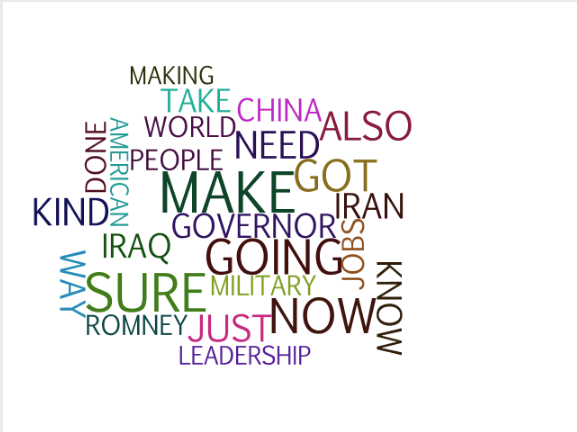
\includegraphics[width=0.7\textwidth]{Moving.png}
  \caption{A Sample Word Cloud - Obama's Third Presidential Debate}
  \label{Makingdupe}

\end{figure}

Several popular word cloud generators exist online, but each follows
a similar algorithm to create its visualization. The following algorithm
is used to create a word cloud:
\begin{lstlisting}
Count the words
Remove trivial words
Sort by the count, descending.
Keep the top N words for some N.
Assign each word a font size proportional to its count.
Generate a Java2D Shape for each word, using the Java2D API.
While(words need to be placed)
  Place the word where it wants to be
  While it intersects any of the previously placed words
  move it one step along an ever increasing spiral
\end{lstlisting}
This pseudo-code was given by Jonathan Feinberg, the creator of the
popular word cloud generator, Wordle. \cite{algorithm} While the algorithm
itself is simple, more advanced elements are required to maintain
speed - Feinberg references last-hit caching, hierarchical bounding
boxes, and quadtree spatial indexes as techniques used to speed up
the intersection test (the generator's bottleneck). 

In the algorithm above, the words selection first needs a number of
preprocessing steps. The text is tokenized (split into individual
words without punctuation) and each word is counted. Next, stop words
- common functional words that add no meaning to the context (i.e.
the, and, a, etc.) - are removed to prevent them from dominating the
cloud. In practice, each word in the list is reduced to its stem to
eliminate duplicates like plurality and verb tenses, and a single
word is chosen to represent this word. From this list, they are ranked
and sized according to their term frequency (amount they occur in
the document) and the first word is placed. 

\begin{figure}[!ht]
  \centering
  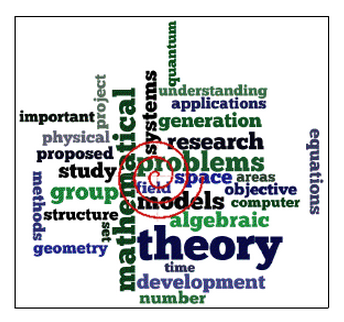
\includegraphics[width=0.7\textwidth]{Spiral.png}
  \caption{Spiral Algorithm from Castella's original paper\cite{Wordstorms}}
  \label{Spiral}

\end{figure}


From here, the algorithm moves in a clockwise spiral and attempts
to place the next word. \ref{Spiral} At this stage, the algorithm checks if there
will be any intersections between a previously placed word and the
current one. This check is performed by hierarchical bounding boxes
since checking the intersection of rectangles
is faster than comparing individual letters. The bounding boxes are stored in
a tree for each word. During the placement section, each descending
node of this tree is checked for a potential intersection. If none
exists, the word is placed and the spiral increments. Once all words
have been placed, the algorithm terminates and a drawing function
is called to display the word cloud. 


\subsection{WordCram}

WordCram is an open source word cloud generator developed by Daniel
Bernier. Its implementation resembles the above procedure for word
cloud creation, with the spiral algorithm and hierarchical bounding
boxes already present in its code. A few notes about WordCram's implementation
are relevant for the rest of the paper: WordCram uses Processing,
a multiplatform imaging tool, as its means of generating the image
containing the word cloud. 

The word storm code, by Joaquim Castella, was integrated with WordCram
- certain functionality was modified to accommodate for the word storm
requirements:
\begin{enumerate}
\item WordCram skips words when unable to fit them within the frame. Rather
than lose information, Castella increases the size of the frame to
allow this word to be placed. 
\item The font size is not set by the word's term frequency. Instead, Castella
calculates a target area for the word to fill. If two words have equal weight,
they are represented on the screen with the same area. By this, Castella
reduces the human tendency to view longer words as more important
- a word with less letters is drawn with larger font to offset its
length. 
\item The layout, algorithm and drawing sections of the code have been separated
to ease any modifications. 
\item The configuration options have been reduced to their simplest form. 
\item The word ranking is ordered by a normalized term frequency. Normalizing
the term frequency reduces the impact of longer documents; crucial
in the word storms project. 
\end{enumerate}
During testing, both the word make and making appeared in a cloud.
This may indicate that the stemming process did not occur, or that
this could be a particular outlying case that needs to be addressed.
\ref{Makingdupe} showcases this problem.

WordCram also features additional algorithms for placing words, but
since Castella's code only applies the spiral algorithm, it is the
only case we consider. Finally, a newer version of WordCram has been
released, and so the methods described in this code may differ from
the current implementation. 


\section{Word Storms}

Word storms are an extension of the word cloud that aim to improve
the analysis of a large amount of documents by using a series of word
clouds. If each document is created independently, the word clouds
are difficult to compare against each other. By placing the clouds
beside each other, and coordinating the appearance across them, the
word clouds can convey more important information faster. This is
the basis for word storms. 

Word storms were created by Joaquim Castella in 2012. In the paper
describing word storms\cite{Wordstorms}, Castella indicates there
are two attributes for gauging a storm's importance. Firstly, each
cloud must be a good representation of its parent document and secondly,
the storm is constructed so that the color, position and orientation
of the same words are shared between clouds. If these metrics are
followed, then the storm will represent each document, and the visual
similarities between the clouds will be easy to see. A user will be
able to evaluate the entire corpora by looking at the overall storm,
compare individual documents through visual similarities/differences
between their respective clouds, and, as with an singular cloud, gain
an understanding of the document.


\subsection{Overall Storm Creation}

The simplest manner of creating a word storm is to run the word cloud
algorithm on each document in the corpora. This, however, produces
none of the desired outcomes from the storm - the documents are difficult
to compare against each other, and the information contains nothing
representing the corpora as a whole. Instead, Castella suggests making
the storm 'homogeneous' - synchronize the orientation and color of any
word which appears in multiple clouds. 

To assist in identifying the important properties of the storm, Castella
manipulates the visual appearance of the words by using tf-idf (term
frequency - inverse document frequency). Term Frequency refers to
the number of times a word appears in the corpora and the Inverse
Document Frequency calculates how rare the word is within the corpora.
By setting the font brightness of words according to their tf or idf
value, the storm can showcase different factors. Using tf highlights
the similarity between clouds, while idf values brighten the documents
that are unique between clouds. According to Castella's paper, the
storm then sets the hue of the word randomly, while the saturation
is constant to prevent dull storms. However, in the code, the values
corresponded to the rgba color model, with the alpha channels relating
to the word's idf value. 

Certain aspects of the word storm are just extended concepts of the
word cloud. For example, the number of words in a single cloud will
be the same for each cloud of the storm. The font typography is shared
across each of the storms to help maintain consistency and aid visual
identification. 

Four different algorithms exist for creating the storms. The first
is the naive approach - generate each cloud independently. The other
three - iterative, gradient and combined - create storms with the
desired similarities and appearances and are considered in depth below.
While the details of storm creation varies depending on the algorithm
chosen, certain factors are common to all in their implementation.
Each document in the corpora is preprocessed - in addition to the
cloud preprocessing seen in a single cloud, the term frequency and
inverse document frequency are calculated for the entire collection.
Furthermore, the coordinated attributes are stored in a mapping between
the word and an object containing all the relevant properties, which
vary depending on the algorithm chosen.


\subsection{Algorthims}

To generate a cloud, Castella employed three different algorithms
to coordinate words across multiple clouds. The descriptions of these
algorithms is taken from Castella et al. \cite{DBLP}. 


\subsubsection{Iterative}

The iterative algorithm aims to coordinate the position of words across
documents. As the name suggests, the algorithm iteratively shifts
the words in the cloud until each word is positioned within a distance
of the others. To do so, each cloud is first generated independently
with the standard spiral algorithm. Next, the average position of
each word across the storm is calculated, and the spiral algorithm
is run again to attempt to place these words near this average. 

The algorithm's speed is improved by relaxing two conditions on its
convergence: the threshold distance for completion is increased if
the storm could not be placed, and a maximum amount of iterations
is allowed before termination. Furthermore, the algorithm won't move
words if they have already converged, and checks to see if, in an
earlier cloud, the word has been placed. If it has, it places the
new word as near to that location as possible without overlap. 

These factors mean that the storm can be generated quickly, but each cloud tends to be sparse. The spiral algorithm
shifts the words away - given enough space, each word can have its
own converged location. But as the distance between words increases,
the cloud's visual appeal and information content decreases. Early
termination limits this effect, but these concerns needed to be addressed
with gradient algorithm described below. 


\subsubsection{Gradient}

The gradient algorithm reduces the sparseness of the iterative algorithm
through a tailored MDS function (titled Discrepancy Between Similarities
\cite{DBLP}). A stress value measures
the relationship between documents and the relationship between clouds
- similar documents/clouds will score low. A correspondence sum measures
how well each cloud represents the document: Finally, a penalty keeps
the words from overlapping and minimizes the word's distance from
the center. The stress value, the correspondence sum and the penalty
are summed together to find the DBS value. Gradient descent is then
used to find the local minimum to optimize the weighted parameters in
the equation. 


\subsubsection{Combined}

The combined algorithm aims to combine the strengths of the iterative
and gradient algorithms. First, the iterative algorithm runs to completion
(either termination or convergence). The gradient algorithm then performs
the MDS optimization, having the effect of pulling the words, spread
out by the iterative algorithm, back together. This gradient section
performs better after the iterative algorithm has run - the words
are optimally positioned for the gradient descent's performance. \cite{DBLP}


\subsection{Implemenation}

The word storm code is layered over the WordCram code. The code
implements a preprocessing stage, where the words are loaded in, tokenized
and stored. The values of the term frequency and inverse document
frequency are calculated, and the index - each word's shared properties
across the storm- is constructed. Once the initial setup is complete,
the chosen algorithm runs. 

In addition to the choice of algorithm, a number of customization
options are provided. These allow the user to manipulate some storm
attributes and are discussed in further detail in section 3.5\ref{sub:Customize-Word-Storm}. 

It is important to note that this is a black box system - the user
provides a folder and a series of images are returned. Apart from
command line modifications (i.e. specifying the algorithm used to
generate the clouds), the way the image files are generated cannot
be modified. This setup hinders any modification to the storms after
their creation. 


\subsection{Usage of Word Storms}

Some of the potential uses of the word storm website are identified
as follows:
\begin{enumerate}
\item Temporal evolution - View the history of a series of documents and
discover how they have changed or evolved over time. For linguists,
one could analyze the similarity of words over time, while a historian
may discover trends in historical documents. In the context of the
web, users can view how their Facebook/Twitter content has evolved
over time.
\item Literature analysis - Determine important thematic elements that appear
in an author's novel (analyzing chapters) or entire work (analyzing
an entire bibliography). In the context of the web, blog posts can
be scrutinized in this manner. 
\item Analysis of Ted Talks \textendash{} By taking the transcript provided
at the bottom of certain Ted Talks, an individual can quickly compare
content of individual videos to identify videos of interest. 
\item Analysis of Critical Works - Summarize a series of critiques provided
by reviewers and compare the similarities to identify the common consensus
about a work (i.e. film, game, or art).
\item Summarize Lectures - Present the core concepts of a year\textquoteright{}s
lecture material into core concepts and identify where common topics
appear. This can be applied to both university level education, or
early schooling years.
\end{enumerate}

\section{Alternatives to Word Storms }

Some work has been done on analyzing and visualizing corpora of textual
data. They are presented here:


\subsection{Collocate Clouds}

Beavan \cite{Collocate} created a different tool to analyze a corpora of documents
- collocate clouds. These clouds, closer in appearance to tag clouds
than word clouds, present collocational relationships between words.
Words are placed in alphabetical order, with brightness and size corresponding
with importance. Though both word storms and collocate clouds are
used to analyze a corpora of documents, collocate clouds focus on
visualizing the context of words within a corpora - which words occur
in the presence of others. Thus, a collocate cloud showcases the word's
relative context, and does not distinguish between the different documents. 


\subsection{Context Preserving Dynamic Word Cloud Visualization}

Cui et al propose an idea similar to the word storm \cite{ContextPreserve} - a series
of word clouds that preserve spatial and semantic relations. They
seek to preserve the context of the word within the cloud. These focus on the evolution of the clouds over time, rather than on the relationships between documents within a corpora. Though the appearance of these clouds may appear visually similar to word storms, the methods used to generate them are different, and do not allow user modifications to the storm. 


\subsection{Word Storm Website}

It should be noted that a 'WordStorm' project is online at www.lonji.net
\cite{Otherstorm}. This project focuses on dictionary entries and the relationships
between words, and has no involvement with the cloud-based visualization
created by Castella or implemented in this project. In the case of
future deployment, a distinction should be made between the sites. 


\section{Web 2.0}

Within the project scope is the requirement that the website be 'Web
2.0'. Given the number of varying definitions for what Web 2.0 is,
defining Web 2.0, and the list of features required to meet this definition,
is essential. Web 2.0 was popularized by O'Reilly Media, and later
defined in an influential paper by Tim O'Reilly \cite{oreilly}.
From this, Web 2.0 was defined a loose collection of concepts describing
the features of websites that survived the dot-com burst. However,
Anderson \cite{web2} clarifies the O'Reilly definition and provides
a definitive list of what Web 2.0 is.
\begin{enumerate}
\item Individual production and User Generated Content - The user provides
the website's value, and determines the behavior of the website. The
website should focus on this user data, and provide context and functionality
around it. Because the users provide value, the ability for them to
create dynamic content should be simple. 
\item Harness the power of the crowd - Large groups of people, acting independently,
can create a unified behavior. This behavior is often self-correcting
and emergent, and is employed to great effect on Web 2.0 websites.
Anderson cites the folksonomy effect as an example of how the crowd
can correct incorrect data. Wrong tags were buried 
\item Data on an epic scale - The large amounts of data that the web has
allowed us access to vast amounts of data. These increasing amounts
of data are processed and analyzed by Web 2.0 websites. 
\item Architecture of Participation - The website improves during a user's
interaction with the website. Furthermore, the site will actively
encourage the user to use the site.
\item Network Effects and the Long Tail - Users will interact with each
other in new and different manners. 
\item Openness - The data gathered is open and accessible. APIs and other
public forums, and the open source movement showcase a trend towards
the availability of information. 
\end{enumerate}

\section{Ruby on Rails}


\subsection{Rails' Strengths}

The project was implemented using Ruby on Rails. By using a framework,
the basic website functionality comes ready-to-use. This decreases
development time, critical in a time-sensitive project. The overall
security of the web site increases - known security exploits are safeguarded
against. With websites like Basecamp, Twitter, and Github running
Rails, the Rails' community is one of the largest web frameworks.
Such a prolific nature enables an easier effort with debugging, and
provides greater support. 

One of Rails' key strengths is its ability to rapidly generate functional
code with minimal effort. This scaffolding code forms the basis for
each Rails application. These quotes, from the Rails website, reflect
the consensus of Rails' speed as one of its strengths:
\begin{quotation}
\emph{``{[}W{]}eb designers and software engineers can develop
a website much faster and more simply'' }- Bruce Perens, Open Source
advocate

\emph{``Powerful web applications that formerly might have taken
weeks or months to develop can be produced in a matter of days.''
}- Tim O'Reilly, founder of O'Reilly Media \cite{Railsquote}
\end{quotation}
The ability to create prototypes quickly and experiment with different
approaches is critical in a time-sensitive project such as this. Choosing
Rails maximizes the time spent on creating the main functionality
of the word storms website, and less time on the less important aspects. 


\subsection{Issues with Scalability}

A well-known issue with Rails is its purported lack of scaling (The
website 'http://canrailsscale.com/' \cite{scaleRails} displays a single 'NO' on it).
With Twitter's high-profile departure from using Rails as a message
queue back-end in 2008, questions arose whether Rails could handle
scaling. In the creation of a scalable website, such limitations must
be addressed before choosing such a framework. With our website, it
does not matter for two reasons: 
\begin{enumerate}
\item Rails Scalability in General - While the common consensus online is
that Rails cannot scale, there are counterpoints to address. Twitter's
front-end still uses Rails and can handle the traffic with minimal
outage. Other high-traffic websites, including the U.S. based video
site Hulu and the YellowPages site, use Rails without difficulty despite
several million users. \cite{Railsscale} The volume of users does not affect the scalability
of Rails. 
\item Twitter's Difficulty Stems from Tweets - Tweets are rapid pieces of
information that require constant updates to the database. Twitter's
global reach also implies that such data must be stored in databases
spread across many locations. To improve performance, websites can
use caching to decrease server load. In Twitter's case, caching would
be rendered ineffective in a few minutes by the influx of data. Contrast
the nature of tweets with the static nature of a word storm. A single
call to the database is required to fetch the word storm, which can
be cached for future viewing. The issues faced by Twitter are inherently
different than the ones faced by the word storm generator, so Rails
as a framework poses little risk. 
\end{enumerate}
Due to the academic nature of this website, it is unlikely that it
will achieve the levels of traffic experienced by Twitter or other
high-profile sites. Such considerations, however, reflect the foresight
required for software development and should be considered
in the case that such a website receives a sudden increase in traffic. 


\chapter{Goals and Requirements Analysis}

In this section, I analyze the project with regard to high level goals.
From these goals, the appropriate steps for implementation can be
determined, and set as the target goals for the project. 


\section{Requirements Capture }

In the Software Engineering discipline, an important step in the creation
of a software project is the requirements analysis. Such an analysis
allows a focus on obtaining the necessary functionalities of the program.
In commercial applications, the application requirements are gathered
from the user - in this academic exercise, without a set of clients
to elicit these requirements, I treated myself as the typical user.
From the requirements, I identified the following goals to reflect
these needs:


\subsection{Adapt Word Storm Code for online usage }

Code for creating word storms was written by Joaquim Castella during
the implementation phase of his project. This code remains much as
it was, though adjustments to the code had to be made. The code was
created with a local implementation in mind, relying on local file
systems and a number of Java jar files. My task was to adapt the code
in such a manner that the functionality of the program remained untouched,
but allowed the necessary customization. Steps had to be taken to
ensure that the code would remain as modular as possible. 


\subsection{Allow Users to Upload Files }

To generate a word storm, the user needs to provide a series of files
for the algorithm to process. In a client-server website, users should
upload their files to the server. The server then performs the computations
and returns a word storm for the user to save or share. 

With a web 2.0 website, the convenience must remain with the user.
Functionality should be guided by the user's expectations and intentions.
Certain behaviors are expected when dealing with files. Users, when
uploading individual files, will expect a standard file navigation
system. Furthermore, it should be convenient for the user to upload
multiple files. If the purpose of the word storm is to generate a
series of word clouds based on a corpora of documents, the entire
corpora should be easily uploaded. 


\subsection{Generate Word Storm }

From the uploaded files, the user should be able to create a word
storm with as little hassle as possible. If the user has uploaded
a series of files, the word storm should be created from those files
and displayed as soon it is ready. If the user chooses an alternate
means (i.e. Twitter user name), the server should perform the actions
to create the word storm without user input. The process should involve
as much automation as possible, to avoid confusion with the user. \cite{dix2004human}


\subsection{Customize Word Storm \label{sub:Customize-Word-Storm}}

Word storms were designed with a number of customization options.
Each of these should be easily accessible to the user \cite{dix2004human} and describe the effects the option has on the storm.
Also, given that the run time can increase dramatically if certain
values are changed (i.e. iteration time), the user should be warned
about the potential duration that it takes to create. Additionally,
these options should not interfere with a casual user's use - these
options should be optional . The possible customizations are as follows: 


\subsubsection{Algorithms}

Castella's code had four algorithms to choose from, which result in
slightly different clouds. The user can select:  
\begin{itemize}
\item Independent algorithm: The naive algorithm that applies the WordCram
code to each storm independently. 
\item Iterative algorithm: This algorithm iterates over possible positions
and slowly shifts the words to a point of convergence across all clouds. 
\item Force algorithm: This algorithm forces a layout based on the DBS gradient
approach. 
\item Combination algorithm: This hybridized algorithm combines both the
Iterative algorithm and the Force algorithm. This is the current default
of the program. 
\end{itemize}

\subsubsection{Number of Words }

The amount of words in each cloud can be set. The default value in
the implementation is 25. The user can choose a number between a maximum
value and a minimum value, depending on performance speeds. 


\subsubsection{Word Angle Synchronization}

The words that occur in multiple clouds will have the same angle by
default. The user can have the option to remove this constraint. 


\subsubsection{Word Color Synchronization}

The color of the words can vary depending on the color scheme chosen.
The current options allow the colors between clouds to be synchronized
or to remain independent. 


\subsubsection{Word Scale}

Each word can be represented by area (reducing the impact of longer
words) or map importance to font size. A binary option allows the
storm to alternate between the two. 


\subsubsection{Tf-Idf Options}

The user can select which statistic to use to color the word. Three
options are allowed - term frequency (amount of times it appears),
inverse document frequency (rarity of the word) or neither (standard
coloring). 


\subsubsection{Font}

The user should have the capability to change the font of the word
storm. However, each individual cloud will not be customizable. The
font selection should take place from a short list of predefined fonts,
with the option to extend it to other fonts in the future. 


\subsubsection{Iterations }

The user should be able to control the number of iterations the word
storm algorithm goes through, as this number will produce different
clouds. The more iterations, the more accurate the positioning of
the words will be, at a cost of time. This trade-off should be customizable. 


\subsubsection{Width/Height of Image}

The final width and height of the individual clouds can be set (to
a maximum value). The user should be able to customize this if they
seek to limit the final size of the Storm. 


\subsubsection{Cloud Positioning}

Otherwise, the users will want to be able to arrange the Word Clouds
in such a manner of their choosing. Thus, the images should be positionable
about the screen and savable in these positions.


\subsection{Scaling Website }

If the amount of users or the amount of CPU stress exceeds the server's
capabilities, the word storm website should demonstrate the capability
to scale. This means that, under duress, additional servers should
be added. The measured performance of the website should not decrease
due to an increase in users. Scalability also prevents complete site
failure.


\subsection{Saving and Sharing }

One of the key elements of the Web 2.0 website is the capability for
users to share information between other users. With word storms,
the ability to share the created storm is a fundamental feature. This
can either be achieved by having a share feature button (which could
send out the word storm as an email), or including a gallery view
where users can showcase a list of previously created word storms.
Once the user is provided with the link, each of the created word
storms can be visible. Privacy options should also be considered when
dealing with user interaction - some users will prefer their information/creations
to remain anonymous. Sharing should therefore remain opt-in. 

Users should also be able to download and save the word storms for
later viewing. This static image, containing the word storm images
in their user-selected locations, should be a PNG to prevent loss
of quality (critical in the case of a word storm composed of dozens
of clouds). 


\subsection{User Login}

To maintain the user preferences described in the previous section,
and to ease sharing between users, the website should feature a user
login system. The user should have a home page dedicated to their
previously created word storms, and have their customization settings
related to their user name. 

This system should also remain secure and provide the functionality
expected of a website. 


\subsection{Testing}

The website should be tested with regard to two overall goals.   
\begin{enumerate}
\item The software should be tested to avoid any software bugs. The standard
practice to ensure this is to build a test suite to test the functionalities
of your code. This involves constructing a series of unit tests to
test individual code segments. There are also automated tests that
ensure the functionality behaves as expected. The web tool Selenium
will provide an additional layer of testing to ensure that each button
on the web page is functional and responsive. 
\item The software should undergo system testing to verify the overall functionality
of the program. These tests will involve stress testing (to test the
capabilities of the database) and scalability testing (to test the
scaling functionality). Both of these require an automated load generator
to quickly create varied data usable for such tests. Therefore, a
sub-requirement of this section is to create a load generator. 
\end{enumerate}

\subsection{Design}

The initial design began as a series of sketched layouts of proposed
user interfaces. To maintain simplicity, the pages chosen for the
project were as follows:
\begin{itemize}
\item Home Page - A page to house all of the navigational links within the
site, as well as provide a brief introduction to the concept of the
word storm. A gallery view of globally shared word storms was originally
intended to appear here. 
\item User Page - A page dedicated to an individual user. A gallery composed
of the user's word storms is the primary focus of the page. The preferences
of the user would also be indicated here (currently only the capacity
for sharing is an option, but further options could be placed here
as well). 
\item Upload Page - Structured as a series of different tabs, each with
a unique method of creating word storms. One tab would be dedicated
to uploading documents, another would allow the inclusion of a Twitter
enter, another would allow for PDFs, etc. Options for customizing
the word storm are presented as a dropdown menu on each of these tabs,
and a button for the creation of the Storm appears at the bottom of
the page. 
\item Word Storm Edit Page - A page that displays the individual Word Clouds.
Each of these clouds is adjustable and there is an option to recreate
the cloud based on a new series of options. 
\item About Page - Page that describes the history of the word storm content,
and a brief description of how the word storm algorithm works. Also
provided are links to relevant sites (Word Storm Github code, Joaquim's
Paper, Word Cram)
\end{itemize}
The actual design of each of these pages should follow the design
of these pages as closely as possible. Smaller details, like the positioning
of the buttons, did not reflect these initial designs. Furthermore,
to aid in navigation, a navigational bar was placed at the top of
the page. The constant presence limits the screen size, forcing certain
designs to be constrained. Additional pages (such as a Login Page/Signup
Page) were also added as needed for basic online functionality.


\chapter{Implementation}

In this section, I will outline the actions taken in the creation
of the web site, and justify their necessity. I begin by discussing
the modifications and additions that I have made to the word storm
code. I outline the website structure and design decisions. I finish
with a summary of the work completed 


\section{Overall Design/Pages}

The final design is represented by a web layout diagram below. 


\section{Word Storm Code}


\subsection{Modifications to Original Word Storm Code}

The word storm continues to be developed and enhanced. Any additions
made in my implementation could not change the core development of
the program. However, certain modifications were made to adapt the
code for remote access. Each of the customization options \ref{sub:Customize-Word-Storm}are
passed to the launcher file - if the prerequisite amount of arguments
is not there, an error code is returned. This helps the server validate
the run time success of the program. A number of other minor functions
were added for ease of access and functionality (i.e. changing the
font was not originally present). 

In the middle of the project, a new version of the code was released
by Joaquim Castella. My design needed only a few minor modifications
to adapt to this new code (mainly to include a call to initialize the
new algorithm).


\subsection{Integrating the Previous Code}

I have packaged the code into a executable jar file. This file is
located within the file system of the Rails code. This code is executed
after the user has pressed the 'Create Word Storms' button. This passes
the current customization options, as well as the necessary file locations,
to the jar file. While jar files conveniently package the code together, 


\subsection{Word Storm State \label{sub:Word-Storm-State}}

Because the word storm code was a closed system - given a file input,
it returned a series of images - any changes to the storm required
generating it from scratch, and then applying the changes. With all the changes 
to the code that would be needed to implement this functionality, I chose to introduce the concept of
state to the storm. The idea is that, once the code has created a
storm, it saves the positions of the words, their colors, their relationships
and the configuration used to generate the storm. From this saved
file, the user can reload it at a later instance and perform modifications. 

To achieve this, I used Java serialization to save the storm object
as a byte file in the target folder. By storing this object, the storm
can be recreated with the necessary attributes (particularly the word
selection), and the files used to originally create the storm can
be removed. This saves the amount of space needed in the server, and
simplifies the uploads database relationship with the user. Serialization
also allowed me to perform changes to the storm once completed (\ref{sub:Additions-to-Word}).

There were three downsides in using serialization. 
\begin{enumerate}
\item Any changes to the storm code or any subclasses renders the object
unserializable - it cannot be reloaded if the code structure has changed. There are two possible
solutions: 

\begin{enumerate}
\item Instead of removing the files, store them and rerun the original code if the file is changed. This increases the storage space required on the server, especially over a given time period. 
\item Introduce versions into the code. If the code has changed, use the version that serialized the code. This is the option I have implemented - the storm is saved in the database with the version of
the code it was created with. Whenever the word storm code has changed,
the newest jar file should be placed into a folder with the new version number. This means that, despite modifications to the storm code, the
serialization process will not break for this particular instance.
This increases server maintenance, and requires users to regenerate
the storm if they wish to access features of later versions. However,
this prevents every storm from needing to be regenerated, and
lessens the amount of strain on the server, as it does not have to
store the files.
\end{enumerate}
\item The precise state is not saved. So any information pertaining to relations
between objects is not reloaded and must be reconfigured. This means
that anything saved within the context of the processing library does
not maintain its state and must be reloaded. 
\item The code itself was not immediately serializable. Each component of
an object needs to be serializable before the object can be. Because
since the WordCram code uses the image library, Processing, the imaging
aspects could not be serialized. To fix this, I refactored the code
so that each accessible object (the WordCram object, the Word object,
the EngineWord object, etc) was serializable. Next, I added subclass
to replicate the code in the processing library - each subclass extends
a particular aspect of the graphics library by calling the super method
(PVector became MyPVector, PGraphics became MyPGraphics, etc). 
\end{enumerate}

\subsubsection{Saving and Loading the Storm}

However, serializing the object at the end of the program, and unserializing
it immediately did not replicate the storm. The positions of the storm
are not saved within the coordinated property, due to the loss of
the relationship with the processing library. All MyPVector instances
within the CoordProp class needed to be written to file and reloaded. 

When drawn, the storm and all word positions are scaled and translated
- the drawing function crops the images to the size of the largest
cloud in the storm, and scales the image to the ratio of 640:480.
Therefore, to preserve the state, the storm's positions are saved
before drawing. However, the words color is set during the drawing
process, so these values must be saved after the draw call. Therefore,
the entire saving process was split into four sections: saving the
word storm as a serialized object, saving the positions of the cloud
to file, drawing the images to file, and then saving the chosen colors.

The resulting files (a color list, a position list and the storm object
itself) are stored in the local file system. These files take up a
small amount of memory - for a storm of six documents, the three files
are comparable to a single image (60 kb). A larger storm with more information 

Reloading the storm requires a number of steps. First, the storm file is
read back into memory. Then, the rendered place and the target place
of each word is reloaded back into the index that relates the word
to a coordinated property. These values represent the pre-drawn values
of the storm. Next, each word in the index has its color reloaded
from the saved file. The configuration of the storm is taken from
the serialized object, and a new MyPApplet (the serialization-correction
subclass used to draw the storm) is created. The storm is reloaded
into the applet, and the defaults are reset. From this state, the
word storm performs as before it was saved - if drawn, the image will
be the same. 




\subsection{Additions to Word Storm Code}


\subsubsection{Moving a word}

I implemented an extension of Castella's code to move a word. After
reloading the saved state of storm, I pass four parameters to the
file. The first value is the pixel coordinates of the word you want
to move. The user can only interact with the image, so these coordinates
are given relative to the scaled 640:480 ratio. The second value is
the pixel coordinates of where the user wants to move the word to.
The third specifies the cloud to manipulate and the fourth specifies
the output folder.

The algorithm converts the pixels into local coordinates (before they
are stretched) by dividing the pixel coordinates by the scale used
when it drew the storm. To find the target word, I iterate over the
list of words in the chosen cloud and check if the pixel value is
within that word's bounding box (the box used to draw the word). The
index then updates this word's values to the target pixels. 

Castella's algorithm then can be applied to these new word locations.
The iterative algorithm corrects any overlapping values caused by
the move, and the gradient algorithm improves the overall appearance,
exactly as before. As a result, our cloud will appear visually similar
to the previous clouds, but the target word will be in the correct
location. 


\subsubsection{Changing the color }

To change a word's color, four parameters are passed. A pixel value,
as a coordinate on the screen, represents the word that should be
colored (found via the bounding boxes). As with moving the word, the
color's input coordinates must be converted to local coordinates.
The second parameter is the color to change the word to, represented
in RGB space. Because the alpha value represents relationships within
the storm (the idf value of the word), I have not allowed the user
to change it. Note that this differs from Castella's original paper,
and does not use HSB. 

Changing the color of a word is simple. Once the storm is reloaded,
the index mapping words to the storm's coordinated properties is accessed.
The color of that particular word is set to the corresponding rgba
value (where alpha is set automatically). The storm is then drawn
with the new color for the chosen word. However, this implementation
assumes that all words are synchronized by color. If the color's are
not synchronized, 

Both of these are created and executed as .jar files, placed in the
same path as the original storm code. These jar files should be subject
to the version required for deserialization. Another constraint
is that the files need to be ordered alphabetically - my code saves
the storm state alphabetically. The cloud id must be set according
to its alphabetical index, or the wrong cloud will be chosen. s

It is possible to call these functions any number of times in sequence
- a user can move one word, color another, and move a third. The state
will remain constant and accessible. However, only a single word can
be moved/colored at once - once the user can only make one change
before the storm is recalculated. 

An series of example images are provided in the appendix to demonstrate the current integration with the website. 

\section{Website Structure and Implementation}


\subsection{Website Architecture}

The code was structured using the Model-View-Controller (MVC) architecture,
something inherent in the design of all Ruby on Rails projects. MVC
architecture divides the code logic into separate sections - the model
contains the data, the view contains the user interface information,
and the controller manages the flow of data between the two. The user/client
only sees the view, and interacts with the controller. The benefits
of using MVC include structuring the code in a logic manner, allowing
modular views that do not depend on the data involved, isolating business
logic from the view, and allowing multiple views to be active
at the same time\cite{Railsstart}. There are only a few drawbacks for using
MVC - it can over-complicate simple projects, updating the controller
almost always means updating the view, and it sometimes can be difficult
to determine where in the MVC the logic needs to be. 

\begin{figure}[!ht]
  \centering
  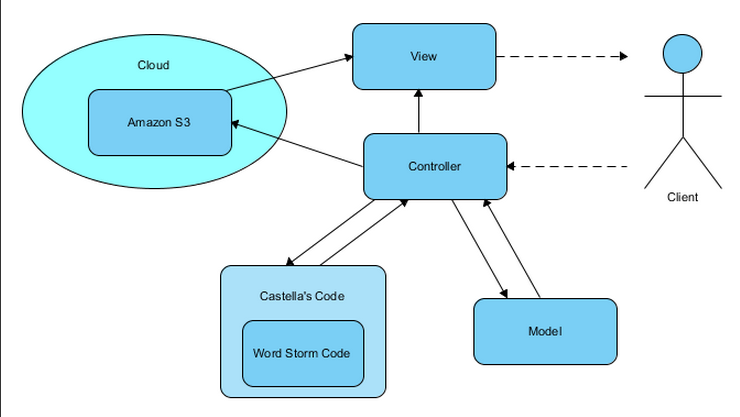
\includegraphics[width=0.7\textwidth]{MVC.png}
  \caption{MVC architecture within the context of my code}
  \label{MVC}
\end{figure}

In relation to my code, I structured it as demonstrated in Figure \ref{MVC}. The view holds my HTML code, the controller contains the functionality,
and the model represents my database (\ref{sub:Database-Setup-and}).
Because the word storm code is contained within a jar file, and is
not included within the main system, I have indicated it's presence
and interaction outside. In addition, the call to 'Amazon S3' is only
in the case of online functionality. In the previous iterations, the
calls to the cloud were represented by a local file system. Toward
the end, the storage service was switched to S3 and is represented
in the diagram as such.


\subsection{Database Setup and Relationships\label{sub:Database-Setup-and}}

The database utilizes Rails' built-in Active Record objects. Each
entry from the database table has a corresponding object associated
with it. Calling the object's methods simulates SQL calls to the database
(Object-Relational mapping), rather than using explicit SQL language.
Beneath this, Rails employs a database management system. Multiple
systems can be used - I initially used the default, SQLite. However,
SQLite does not provide adequate scaling - each read to the database
locks the entire database file \cite{sqlite}. To prevent issues with multiple
users accessing the database at the same time, I chose to change the
database system to PostgreSQL. 

Swapping the system was trivial, due to Rails' abstraction of the
database. PostgreSQL provided a few additional features, the most
important of which allowed the Ruby Gem ``Rubber'' to autodeploy
the website to my EC2 instance (\ref{sub:EC2}). PostgreSQL also provides
backups, general support for scalability, security (a user name and
password are now needed in the database.yml file to run) and a greater
number of features. These attributes ease maintenance and future development. 

I created three different Active Record objects (User, WordStorm,
Image), and used two others (Uploads and Settings), adapted from online
code. Each active record object has, by default, three values - an
auto-incrementing ID for each entry in the database, and two date times
(Created\_At and Updated\_At) for when the entry was created and when
it was last updated. 


\subsubsection{User}

The User object represents the individual using the website. A database
entry is created when the user signs up (a mandatory action to use
the website by design), with a user name and an email. The password
is stored as a salted encryption (to prevent both rainbow table attacks
and reading the unencrypted value in the case of an security attacker)
and verifies the user upon logging in. The storm\_num value represents
the amount of storms that the user has created, and is used in the
creation of a unique filepath for each storm. For security, user names
and emails must not have been entered before, the password is stored
as a salted hash in the database, and a password confirmation is required
before sign-up is allowed. 


\subsubsection{Uploads}

The Upload object represents the files uploaded to the server. This
was sample code taken from JQuery Sample application \cite{Jquery}. The upload contains a
name, content\_type (in our case, always restricted to text), and
size of the file. The entry is only created once the file has been
successfully uploaded - if there is an error with the server, or the
user cancels the upload before . These entries can be deleted once
finished, and are automatically deleted once the word storm has been
created. Further information can be found in \ref{sub:Uploading-Files}. 


\subsubsection{Settings}

The Settings object is created via the ledermann-rails-settings gem \cite{ledermann}. This integrates with a Active Record object and
allows the settings to be set without creating an entry in the database.
Further settings can be added without needing to perform a migration
(adding new columns to an existing database table), allowing for user
settings to be added by default. 

Here, each of the customization options used in the storm generation
are saved as part of the user's settings. When a new user is created,
these values are set to the defaults (the original values found in
Castella's code). 


\subsubsection{WordStorm }

The WordStorm object represents the individual word storm. A database
entry in this table is created whenever a user successfully generates
a word storm. The file location represents where the data files and
image (if not using Amazon S3 (\ref{sub:S3})) associated with the
word storm are located. The name is a user chosen name to describe
the storm (defaults to 'Untitled'). The size represents the width
of each cloud when displayed in the gallery. The height is calculated
via the width to maintain the 4:3 ratio (i.e. full size is 640:480).

The version value indicates the version of the word storm code used
for creation. This is my method of solving the backwards compatiability.
If the storm's state wants to be accessed, the file system will look
in the folder with the version number and call the code from there. 

The algorithm represents the the manner in which the storm was generated
- certain storms have different properties than others. The algorithm
value is used to check if a particular storm can be colored or manipulated. 


\subsubsection{Image}

The Image object represents the individual word clouds. A database
entry is created for each unique image/document in the word storm.
The file location represents the individual path for the image - this
can either be the value of a . Pos\_X and Pos\_Y values represent
the draggable positions of the image within the storm. 

The user has several associations to maintain the relationships between
the tables, and to ensure the correct information is updated during
creation or deletion. A user has many uploads and many word storms
(has\_many relationship specified in the model). Each word storm and
upload can only belong to one user (belongs\_to relationship), and
a word storm has many images (has\_many relationship). An image belongs
to a single word storm (belongs\_to relationship). 

The complete graph of the dependencies can be seen in the following
entity-relationship diagram (Figure \ref{ER}). 

\begin{figure}[!ht]
  \centering
  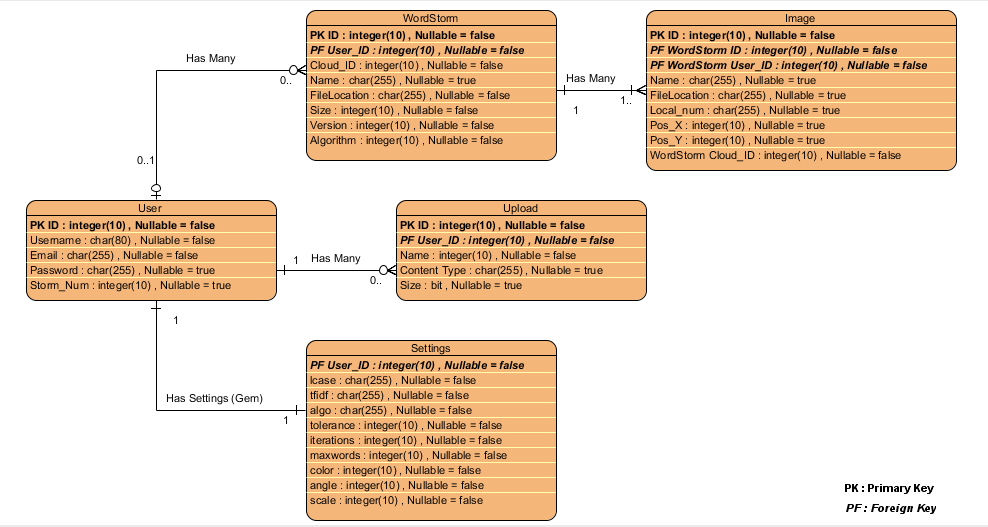
\includegraphics[width=\textwidth]{Er.png}
  \caption{ER Diagram for the database}
  \label{ER}

\end{figure}


\subsubsection{Storing Files}

Neither the files created to save the storm's state (\ref{sub:Word-Storm-State})
nor the images are saved in the database. These files are either stored
in the local file system or on the cloud. This was done under the
initially assumption that databases would suffer from performance
issues when loading images \cite{StoringDB}. However, research from Sears
et al. \cite{Blob} suggests that BLOB (binary large objects - images
in this example) under 256KB perform better in the database. Because
of the large amounts of white space in each of our images, the file
sizes do not typically exceed that amount (this is dependent on the
algorithm used, font choice, letter case used, and number of words
in a cloud). The images could be stored in the database from this
paper's findings. 

However, the paper also suggests that fragmentation resulting from
storing a file long-term is easier to handle by the file system. Additionally,
the database management system would need to be maintained - the relationships
between the images in the database and the original storm needs to
be preserved in the database itself. Storing the images online also
reduces the strain on the server's bandwidth. 


\subsection{Javascript}

JQuery and, by extension, Javascript are used extensively within the
word storm website. If Javascript is disabled, the site could break
when dependent on Javascript. To avoid this, each page checks for
the presence of Javascript,. If not found, the user is directed to
a page asking them to reenable Javascript before proceeding. Rather
than provide the user with some functionality, and provide a potentially
faulty service, I chose to disable the website. I have justified this
in accordance with Shneiderman's Golden Rules \cite{dix2004human} - the interface should
be consistent. If the website works for some sections, and not others,
the usability suffers. In my implementation, the use is consistent. 


\section{Users}

Users are required to sign-up to generate a word storm. This design
helps maintain the file structure for both uploads and created storms.
To sign up, users provide a user name, password and email for the database.
Upon signing up, the user is given the default list of preferences.
These represent the customizations available for the storm and can
be seen on the profile page.


\subsection{Profile Page}

Users have their own homepage associated with their user name. This
page displays their information, along with their preferences for
customizing the storm. The preferences are saved whenever the user
navigates away from their page. The profile page is only accessible
by the user currently logged in. This page also contains a link to
view the user's storms and a link to generate a storm, to assist in
navigation. 


\section{Uploads}

The uploads page is comprised of three tabs. The first contains the
primary functionality - the ability to upload text files. The second
is a proof-of-concept Twitter generator that creates a storm from
a Twitter user name. The final tab gives the user a list of options
to customize the storm. 


\subsection{Uploading Files\label{sub:Uploading-Files}}

Single file upload is a trivial issue - many different versions exist
online. However, word storms require a corpora of documents to function
effectively. In the case of a hundred files to analyze, users will
not want to individually upload each file, so alternatives must be
considered. Uploading files should provide a high level of usability,
due to its relevance of the application. Several methods were considered
for users to upload their files:
\begin{enumerate}
\item Zipping the Files - A singular file upload can be used if a zip is
passed to the server. However, the contents of the zip need to be
verified, the user is inconvenienced by needing to zip the files beforehand
\cite{dix2004human}, and the server needs to spend time unzipping
the file. For these reasons, this was discarded. 
\item File Transfer Protocol - Either standard FTP (File Transfer Protocol)
or SFTP ( SSH File Transfer Protocol) could upload the files. Using
FTP can potentially open a number of potential vulnerabilities to
the server (including bounce and spoof attacks) while SFTP requires
additional setups for the authentication and a public key system for
each user. If security was a priority, I would have chosen this method. 
\item JQuery Uploader - A Ruby gem that allows for simultaneous file upload.
As a gem, its functionality has been secured, verified and tested.
It provides a simple user interface (showcases the progress for the
upload), and does not require flash. The files are displayed on screen
using an AJAX call, providing users with visual feedback for their
interaction with the system. This interaction provides a higher level
of usability, with regard to 'Shneiderman's Eight Golden Rules' \cite{dix2004human}. Because
of these reasons, I have used this uploader. 
\end{enumerate}
The uploaded files are stored in a database with a dependency on the
users. The files are limited to text files, due to the constraint in
the original code base. At present, the contents
of these documents are not checked for malicious code, due to a lack of 
data about the feasability of the attack. This potential attack vector should be investigated in the future, especially within the context of how WordCram processes the text. 


\subsection{Twitter Scraper}

To ensure extensibility, I have designed the website to allow alternative
means of uploading documents for storm analysis. As a proof of concept,
I constructed a Twitter Scraper to create a storm from a Twitter user name.
I access the Twitter API and fetch a list of the user's tweets (up to
a limit of 200 as per Twitter's design) as an XML file. I then parse
the file for the Tweet's content. Because each Tweet is limited to
140 characters, the resulting storm is a large number of clouds, each
containing little information. 

To gain more meaningful clouds, I grouped each tweet by month. However,
this posed a problem for individuals who tweet quite often - the BBC,
tweeting around thirty times, has one or two clouds created before
Twitter's access limit is reached. Instead, I limited the amount per
cloud to thirty tweets, an arbitrary number to divide the clouds \ref{Twitterexample}. Further
refinement would require preprocessing (i.e. calculate the average
number of tweets per month and divide the clouds accordingly), but
this serves as a proof of concept. 

Integrating further scrapers/uploaders into the code is trivial. Possible
extensions, or a Ted Talk scraper) would either need a new upload
page (i.e. a PDF uploader) or a new scraper (i.e. enter a web site
URL and scrape the data). The files gathered only need to be preprocessed
into text files before they can be analyzed as a word storm. 
\begin{figure}[!ht]
  \centering
  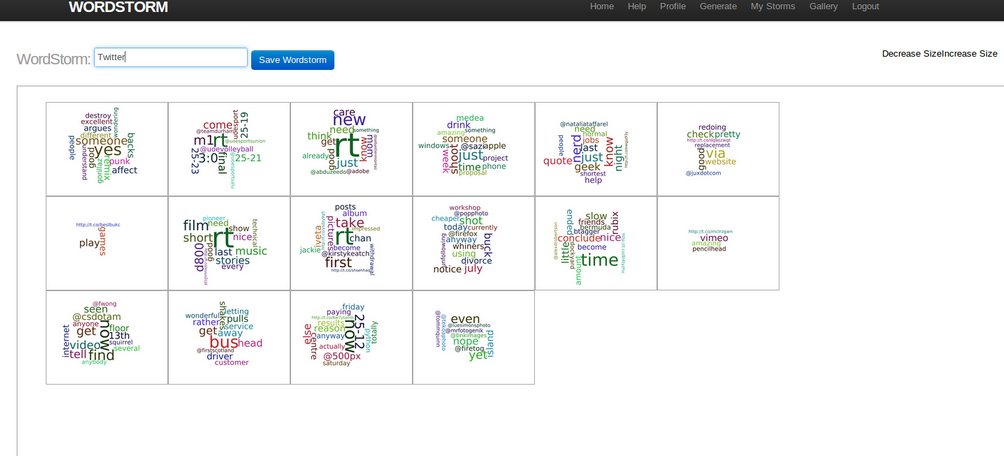
\includegraphics[width=0.7\textwidth]{Twitter2.png}
  \caption{A sample Twitter page generated.}
  \label{Twitterexample}

\end{figure}

\subsection{Customizing the Storm}

To customize the word storm, the user is presented with a tab of the
customization options listed in \ref{sub:Customize-Word-Storm}. The
tabbed menu allows for casual users to generate a word storm as simply
as possible \cite{dix2004human}. The settings reflect the user's
preferences, and are, by default, the standards defined in the original
word storm code. 

These options are presented as a series of number forms, menus and
buttons. This simplifies the understanding By presenting the information
in this manner, the user does not have understand what are a range
of suitable numbers or selections. This allows them to use the word
storm without having to understand the precise implications of each
of the options. Furthermore, to clarify the understanding, hovering
over the individual options provides an in-depth analysis of the functionality. 


\section{Creating the Storm\label{sec:Creating-the-Storm}}

After the files have been uploaded, the required options are passed
to the jar file (input and output locations, and customization options)
and the word storm code is executed. If the results are okay (the
files are found, and the image can be created), the word storm is
added to the database. Each of the created images is also added to
the database with the default size and positions set. 

The user is directed to a page where the results are displayed. This
is a collection of thumbnail images arranged in a series of JQueryUI
draggable boxes. By default, the items are positioned equally across
the screen, but can be dragged by the user to any position within
the containing box. When the images are clicked, their contents are
displayed as a large box in the center of the page using the Lightbox
JQuery plugin by Lokesh Dhakar \cite{LightBoxLink}. Users can view the
individual Word Clouds this way (and save them to their local file
system if desired). 

\begin{figure}[!ht]
  \centering
  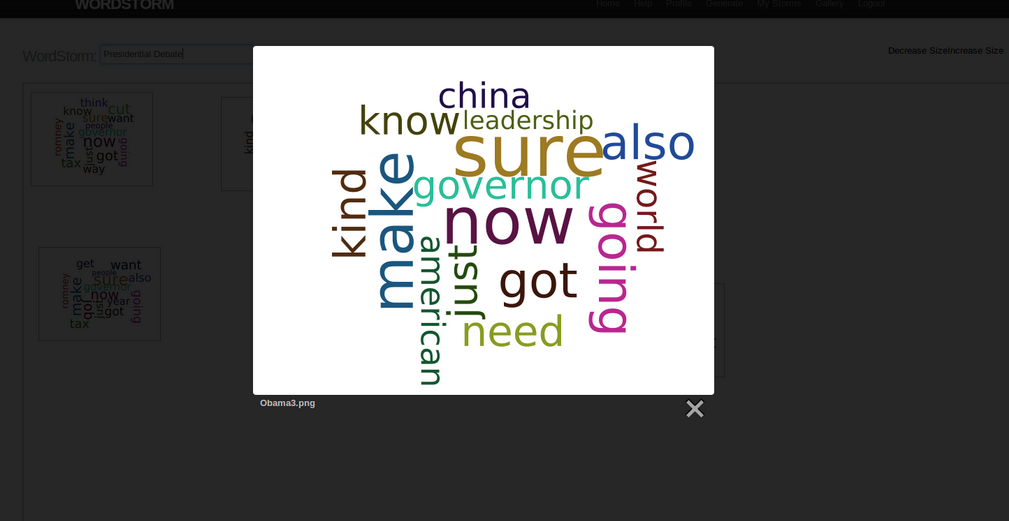
\includegraphics[width=0.7\textwidth]{Lightbox.png}
  \caption{LightBox displaying the image in the center of the page}
  \label{Lightbox}

\end{figure}

The draggable images can be resized using an 'increase size' and 'decrease
size' button. Pressing these buttons changes the size of the image
while maintaining the 4:3 aspect ratio (the values are bounded between
640:480 and 100:75). 

Two further edits are available when the image has been opened
in Lightbox. If the user presses the left mouse on any word and then
again, the word at the first click will move to the position of the
second click. If the user presses the right mouse on any word, a dialog
prompts for three color values (rgb). Pressing okay will color the
word at the clicked location to the chosen color. If the user clicks
on a location where no word exists, the code is still executed, but
an error will indicate that no word could be found. These functions
are called via jar file, under the same version system as the original
storm code. Once the edits have finished, the page is refreshed and
the new images are displayed. 

Finally, the storm can be saved with a unique name. Once saved, the
positions of the clouds are saved to the database and the user is
directed to a page where they can view their storm. 

Once the storm has been created, the files uploaded to the server
are removed. This is done for two reasons. The data is no longer needed due to the serialization - all the information needed is contained within the serialized file. These uploaded files only take up space on the server. 

\section{Viewing the Storm }


\subsection{Gallery Layout Page }

There are two different layout pages for viewing storms. Both galleries
check to ensure that at least one storm is available for viewing before
displaying. If a storm is not available, the user is redirected to
the upload page and prompted to create a storm.

All images in the gallery can be clicked to view the storm as a LightBox
modal dialog. However, the functionality to move/color a word is not
allowed. 


\subsubsection{User Created Storms}

The first is a gallery of the user created storms. This page allows
the user to view their created storms, and access the editing page.  


\subsubsection{All Storms}

The second contains a list of all the storms that have been created. This gallery shows
the storm's name, and the user who created the storm if the privacy
settings allow it. A cookie is used here to maintain the position,
so that, if the user exits and returns, the storm they were previously
viewing is reloaded.
By including this function, users are able to view other user's storms. This was done to foster the user-driven, emergent behavior of Web 2.0. A user analyzing the storm may discover new insights, or use the storm for their own project. A gallery view facilitates this discovery. 


\subsection{Sharing the Storm }

When the share function on either the user's gallery page or universal
gallery page is pressed, the user receives a prompt to enter an email
address. Upon submitting, the email address is verified via both a
regular expression and the Sanitziation gem, and an email is sent
to the target address. The server needs to have smtp configured for
this to work (i.e. postfix on Ubuntu). Using email to share storms
increases the reach of the storms and provides a level of familiarity
to the users. \cite{Infograph}


\subsection{Editting the Storm}

A link from the user's gallery page allows the user to edit the storm.
The edit page allows the user (and only the user who the storm belongs
to) to manipulate the storm. The edit page is the identical to the
creation page.


\section{Scalability}

To achieve scalability in this project, two methods were looked at.
EC2, Amazon's virtual servers, are created on demand as customizable
instances. The goal of using EC2 was to allocate the necessary servers
needed for this project, and increase them as needed. EC2 allows customization
of the server size, number of servers that work in conjecture, and
the operating system specifications for each server. Amazon provides
load balancing to ensure that each instance receieves an equal amount
of traffic. 

The second, S3, is Amazon's online storage facility. The storage itself
is scalable - the amount of storage needed will increase upon demand.
It also provides a level of security. S3 represents its overall structure
in a bucket. Information can then be pushed to and fetched from this
bucket using S3 requests. These requests decrease the bandwidth cost
on your server by shifting the load to Amazon. 

By using Amazon's services, the information is provided online and
accessible from multiple locations. The cost depends on your use,
and a servers can adjust to cope with an increase in useage. The size and useage of Amazon's data services ensures that the software provided is maintained, available, and the
latest security features are implemented. Both the EC2 instances and
the S3 bucket were created from Amazon's Ireland location, and must
be accessed from these locations. 


\subsection{EC2\label{sub:EC2}}

EC2 allows websites to add instances of a particular server when needed.
Each server would perform a specific operation - one would act as
the database, one as the web portal, and the other as the application.
If the load increased on the database, the database could replicate
and horizontally scale by adding another database. This database,
a slave to the original, would decrease the load undertaken by the
master. A load generator performs this switching functionality. 

To deploy a Rails application to EC2, a gem called 'Rubber' can be
used to deploy to the instance using your Amazon credentials. Each of my servers - application,
database, and web - ran an Ubuntu instance provided by alestic.com. 


\subsubsection{EC2 Issues\label{sub:EC2-Issues}}

After deployment to EC2, the instance's permissions prevented the
client from uploading files to it (the user needed write permission).
Each time code is deployed to EC2, a mounted directory is created
with new file permissions. I would have modified the deployment mechanism
to automatically set permissions, but had a larger issue not taken
priority. 

When attempting to generate the storm from the uploaded files, the
Processing library threw an 'X11' error because it needs a display
to generate images. The Processing library cannot run without this display. I managed to run the code by calling a frame
buffer (xvfb), but this doubled the runtime for a small sample (three
documents), and introduced a number of potential security flaws (with
regard to necessary permissions to execute). Furthermore, the files
required for the frame buffer to work doubled the server's size to
3GB of the 7GB provided. Each new instance would need to undergo this
configuration when being added. 

As a result, the code was taken down from Amazon EC2 and the instances
torn down. In my opinion, the issues were not worth the added concerns.
I could not find other alternatives for running Processing on a headless
server. Instead, I would contend that, if the website wants to use
Amazon's EC2 instances, then the foundation for the word storm - WordCram
- needs to be refactored to not require graphical memory to use. The
time commitment involved in the large-scale refactoring of the codebase
was deemed too great. The EC2 code, however, remains in the code in
case of future use. 


\subsection{S3\label{sub:S3}}

Instead, I used S3 to host the images online. Once the images are
created from the storm, each of the files is pushed into an S3 'bucket'
via the S3 gem. The bucket is structured in the same style that the
original file system used - each user has a folder within a bucket;
each storm has a folder inside that user's folder. Upon successful
upload, the word storm is created as normal (the path still points
to the local file system).

Each of the image database entries are modified - their file location,
instead of pointing to a local file, points to an amazon URL (i.e.
https://s3-eu-west-1.amazonaws.com/wordstorm.bucket/1/8/...). When
the user looks at a storm, each of the files is fetched from the Amazon
servers. This reduces both the bandwidth required by my server and
the amount of file storage needed on the local server. Because the
storage will increase due to the demand, the file system can be considered
slightly scalable. 


\section{Security }

The Open Web Application Security Project (OWASP) has published their
list of the top ten security faults on the internet in March 2013
\cite{OWASP}. Although only an interim report, the contents provide insight
into popular attack vectors and methods to safeguard a web application.
From this, I have addressed a number of security attack vectors and
discuss how they have been protected in the word storm website. 
\begin{itemize}
\item 1) Injection - An attacker exploits the code intrepreter to insert
his code into a request. Rails, in certain regards, provides security
for this. However, for any value that the user can potentially modify,
I use the Sanitize gem to secure the input by removing unsafe elements
(HTML code, SQL code, etc). 
\item 2) Broken Authentication and Session Management - An attacker exploits
poorly managed sessions or authentication. To prevent an exploits,
the session expires after one hour, and the password is stored in
a secure manner (as a salted hash). 
\item 3) Cross-Site Scripting - The attacker exploits the browser's intrepreter
to execute code. The Sanitize gem is used on textual input, and the
parameters passed via post are checked for validity. 
\item 4) Insecure Direct Object References - The attacker gains access to
unsecure data by posing as another user. To prevent this, the user
is required to log into the word storm website. All of the data provided
(personal storm access, uploads, settings) is only accessible via
this account. 
\item 8) Cross-Site Request Forgery - The attacker forges an HTTP request
and submits their own form data. A crsf\_meta\_tag inserts a crsf\_param
and a crsf\_token on each page, to add an identifying signature for
it. Whenever a form is submitted, these values are also submitted.
Upon receiving a form, the values are checked to confirm where the
request came from. If the request does not match, the form data is
discarded. 
\item 9) Using Components with Known Vulnerabilities - A website component
in the design has known flaws. Rails had several security breaches
in January 2013 \cite{RailsSec}. By upgrading my version of Rails, the attack
vector is removed. Additionally, I have switched to Thin as a web
server instead of WEBrick. - WEBrick displays potentially compromising
information within the HTTP response. 
\item 10) Unvalidated Redirects and Forwards - The attacker exploits the
automatic redirect to another site. I check each parameter during
a redirect, and ensure the user is still logged into the application
before accepting a redirect. 
\end{itemize}
Number 5 (Security Misconfiguration), Number 6 (Sensitive Data) and
Number 7 (Missing Function Level Access Control), while important,
were not directly addressed directly in my application. While certain
security flaws may still exist within the application, a basic level
of security has been implemented. 


\section{Legality}


\subsubsection{Cookies Useage }

A Rails session id is used to maintain a user login. An additional
cookie is used for the gallery page to maintain viewing position.
In June 2012, Article 5.3 of Directive 2002/58/EC \cite{cookie} was
drafted by the EU Directive on Privacy and Electronic Communications
to safeguard user data. In compliance with these new regulations,
a warning detailing the use of these cookies is given at the forefront
of the website. The implicit consent of the user, and their agreement
to the use of cookies, as outlined by the Information Commissioners
Office\cite{cookie}, complies with the legal requirements of this
directive. The session id performs in accordance to this law and expires
1 hour after user login. 


\subsubsection{Data Protection Act}

The Data Protection Act of 1998 \cite{dataprotect} regulates personal data if
any indentifing information is contained within. Data, by the Act's
definition \cite{dataprotect}, is any information which is processed. By reading
and tokenizing the uploaded files, the storm website processes the
information and thus any uploaded file is considered data. 

Personal data, by the Act's definition, is any information that can
identify a user. The website cannot know if the user information is
personally identifiable - the information may or may not contain sensative
information and could identify the user (names, locations, or other
information). Data from a Twitter stream, or the uploaded textual
documents, in conjecture with the email address used to sign up, could
identify an individual under certain circumstances. Due to the user
requiring an account to upload storms, the information is linked with
their username, thus holding them accountable. 

Due to the situation where an individual can be identified by this
data, the Data Protection Act should be followed. In this case, we
can assume consent to process the files has been given by the user's
upload. In accordance with the Data Protection Principles, the data
must be adaquately safeguarded, and the information contained within
cannot be extended to outside the European Economic Area (unless the
area in question is secure)\cite{dataprotect}. 


\chapter{Evaluation}

This section details the evaluation of the website. For the implementation,
I compare the features implemented in the final version of the website
against the initial requirements outlined by both the project specification
and my own requirements analysis. I then indicate areas where the
project can be furthered. 


\section{Comparison Against The Project Specification}


\subsection{Word Storm Website}

At the project completion, a functional website has been created. A user can access the web page, upload a series of text files in sequence and generate a word storm from the resulting files. The storm is fully customizable - a number of options are provided to the user upon storm creation. These include all of the requirements defined in \ref{sub:Customize-Word-Storm}
While the original idea to share the storms was implemented, the privacy action was not. 

\subsection{Screenshots}
Here, I have provided a number of screenshots demonstrating the code's current appearance and functionality. 


\begin{figure}[!ht]
  \centering
  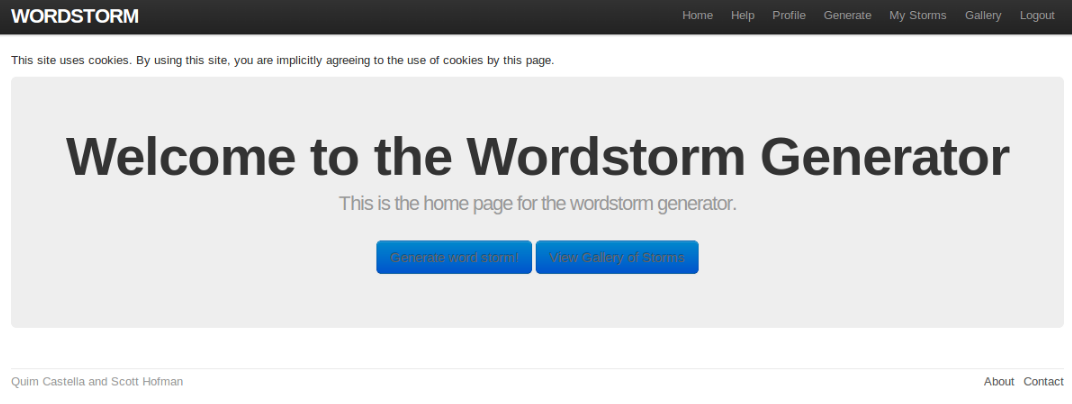
\includegraphics[width=0.7\textwidth]{HomePage.png}
  \caption{The home page of the storm}
  \label{Homepage}

\end{figure}


\begin{figure}[!ht]
  \centering
  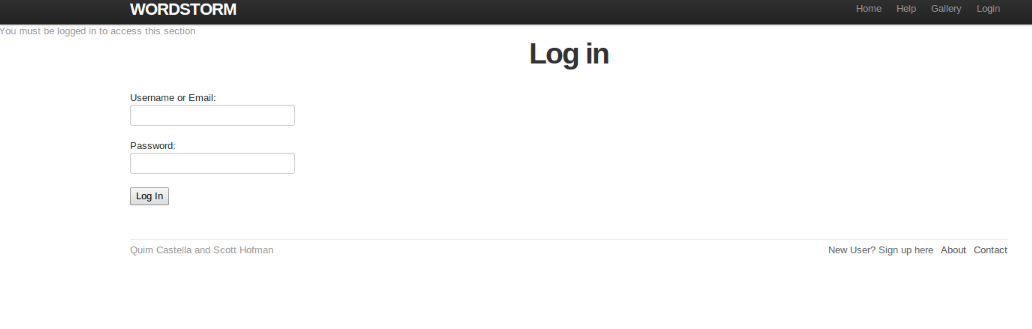
\includegraphics[width=0.7\textwidth]{LoginVerify.png}
  \caption{The log in screen}
  \label{Login}

\end{figure}



\begin{figure}[!ht]
  \centering
  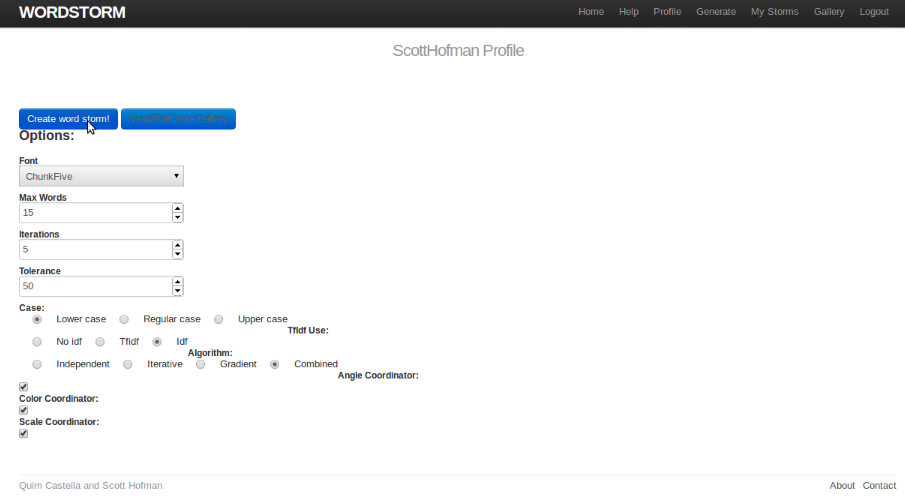
\includegraphics[width=0.7\textwidth]{Profile.png}
  \caption{The profile page, with a list of all the available settings}
  \label{Profile}

\end{figure}



\begin{figure}[!ht]
  \centering
  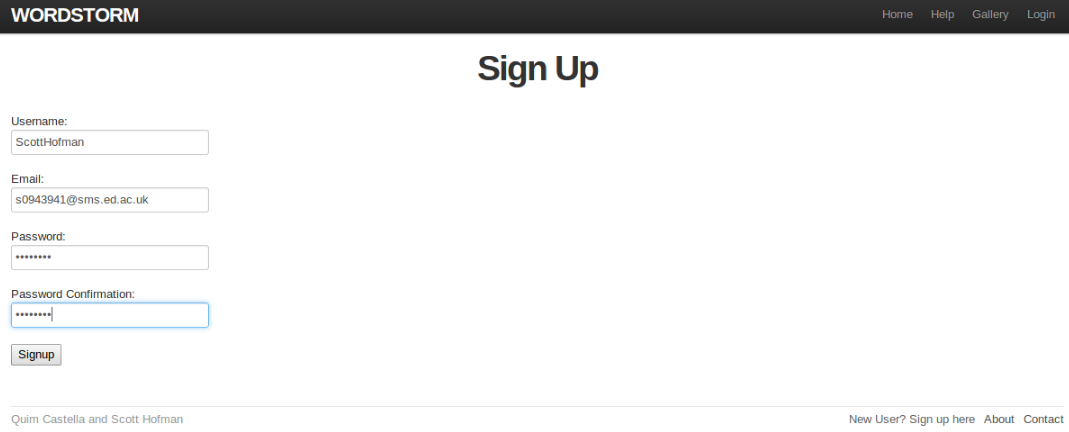
\includegraphics[width=0.7\textwidth]{Signup.png}
  \caption{The signup page to allow users to access the website}
  \label{Signup}

\end{figure}


\begin{figure}[!ht]
  \centering
  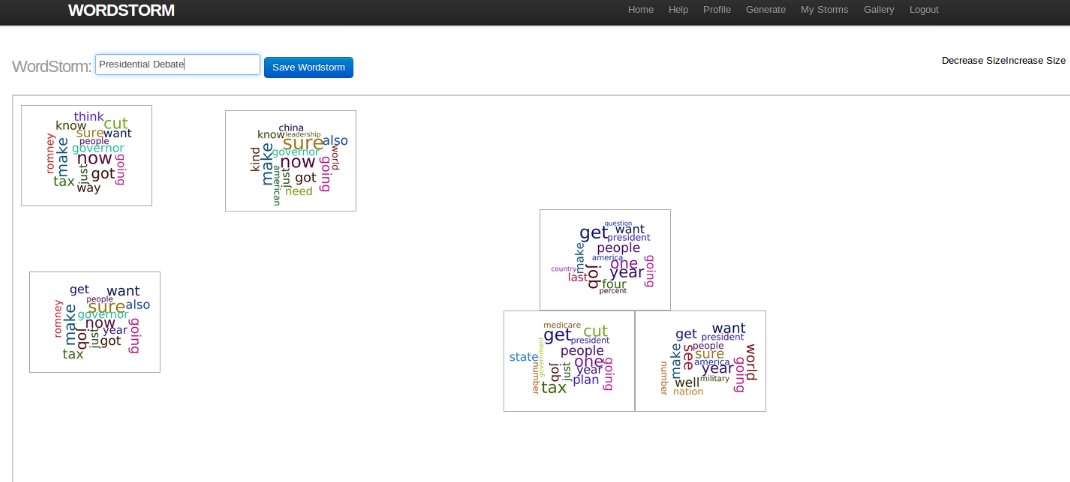
\includegraphics[width=0.7\textwidth]{Storm.png}
  \caption{A completed storm - showcasing the Presidential Debate.}
  \label{Storm}

\end{figure}


\begin{figure}[!ht]
  \centering
  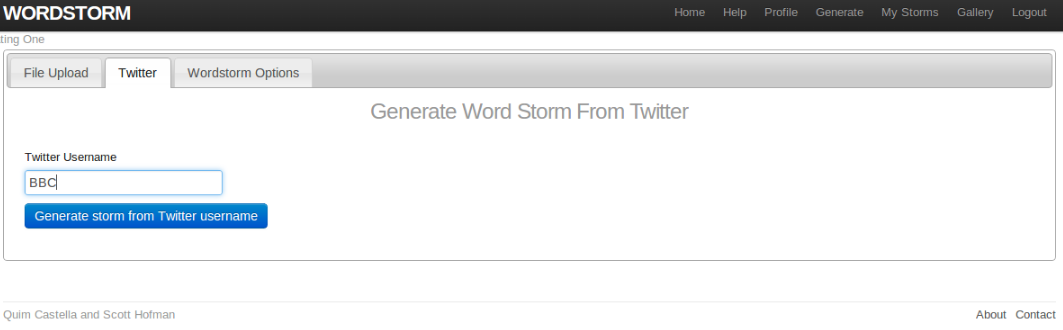
\includegraphics[width=0.7\textwidth]{Twitter.png}
  \caption{The conceptual Twitter plugin, allowing users to create a word storm from Tweets}
  \label{Twitter}

\end{figure}


\begin{figure}[!ht]
  \centering
  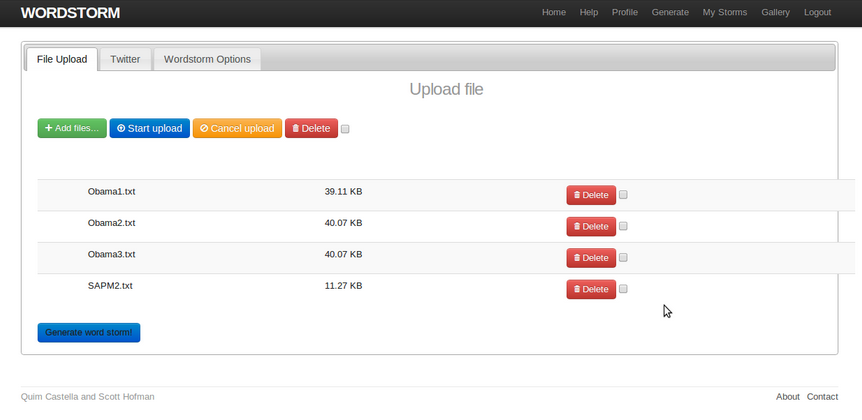
\includegraphics[width=0.7\textwidth]{Uploads.png}
  \caption{The page allowing the users to upload files}
  \label{Uploads}

\end{figure}

\subsection{Web 2.0}

With regard to the six principles defined by Anderson \cite{web2}, the Word Storm's
website fulfills four through the project's implementation. The word storm's purpose of processing and evaluating data, when applied
to the web, translates to the data-processing concept of Web 2.0. To use the
storm, the user must upload files and therefore provide content. All value must come from the user in this design. From
this content, new information (the storm itself) is generated. With the code available on Github already, a certain level of openness is fulfilled.
To achieve the desired network effects, I have implemented sharing functionalities. The ability to both view other users' storms and email a specific individual increases the sharing potential within the network. 
The last points - architecture of participation and harness the power of the crowd - depends on the level of attention that the word storm website receives. If many users are creating storms, then the website's functionality is expanded. This will, in turn, draw more users to the website and create more content. From this generated content, if the users are able to draw information from the application, or upload a version of the storm that better represents a corpora, then the power of the crowd will improve the quality of the information within the website. However, these require a physical deployment and long-term testing to analyze and verify. 

\subsection{Scalability}

The scalability metric was not achieved to the required level of specified at the start of the project.
While the website could be deployed to EC2, the server configurations
could not be customized to allow the word storm code to run without
configurations that limited its effectiveness. If the project wants
to use EC2 (or any server without a graphical display), either the
word storm code needs to be changed or another workaround needs to
be found. 

A small scale level of scalability was provided by the inclusion of
Amazon S3. Amazon S3 increases the size of the storage provided. Additionally, Amazon's servers, rather than the local ones, would bear the brunt of the load in the case of increased traffic - their servers would need to adapt to deal with the increased traffic. 

Furthermore, other aspects of the design were changed to allow for the design to be scalable. The database PostgreSQL allows for scalability customization - if the database reached a critical level of use, another database could be replicated as a slave to the original. The code for EC2 deployment is also within the code, and can be used once the storm can be generated without a display. 

\subsection{Additional Criteria}

Certain criteria was not outlined in the original topic, but were
implemented as additional work. Saving the state of the word storm allows for a decrease in the storage requirements, and eases the ability to modify the storm after generation. Additions to Castella's original algorithms allow the moving and coloring of individual words, in the case that the storm needs minor adjustments. A proof of concept generator from Twitter showcases the websites ability to extend and adapt to reflect the desires of its Web 2.0 users. 


\section{Future Work}

There are a number of possibilities for future work with the word
storms website:


\subsection{New Algorithms}

Joaquim Castella and Charles Sutton's new algorithm for generating
word storms reflects the potential for new algorithms to be developed.
These algorithms could be introduced as alternative options for generating
the storm. Another useful feature would include the ability to introduce
a new document into the corpora, and have it update without being
forced to start the algorithm from scratch would be useful for any
long term prospect of the word storm. 


\subsection{User Testing}

Long-term user heuristics could illuminate both the manner in which
word storms are used, and, with regard to usability, how the website
performs. From these results, certain features could be added, redesigned
or removed from the website. 


\subsection{Different Display Mechanisms:}

Currently, the word storms are displayed on the screen without any
relation between the clouds' positions. While the user should still
be able to customize their position, it might be revealing to have
the initial location reflect metrics between the clouds themselves
(i.e. similarity measure between two clouds represented by distance
between the words). By having this as an option for positioning/default,
and have different metrics for comparing clouds, the position can
add another dimensionality to the word storms. 

Users may want to be able to combine different clouds together, or
create subsets of storms. These would need independent display mechanisms,
and different methods for achieving this. 


\subsection{Improve/Extend Information Gathering}

As mentioned in section 5.8, the Twitter scraper suffers from the
inability to be customized relative to the number of Tweets a user
makes. Additionally, the web has a large amount of potential information
sources that can be visualized within a word storm (i.e. different
sections on Wikipedia, TED talks, university lectures), but the website
lacks the necessary capability to parse the data. Finally, word storms
can only process .txt files, and so cannot deal with the majority
of the information on the web. Changing the input process, by including
both the ability to deal with .pdf or .doc files and adding scraper
to popular websites increases the number of potential usages. 


\subsection{Refactoring the Codebase}

Two issues encountered during the implementation of the project -
serialization and EC2 errors - were the result of limitiations in
the Processing Library. While there are methods around these limitations,
these hacks hamper the project's extensibility. The project is highly-coupled
- WordCram relies on the Processing Library, Castella's word storm
code relies on WordCram and my code now relies on the word storm implementation.
For the project to continue to evolve, and adapt (run on a headless
server), the codebase should be refactored to remove the coupling
and provide alternative means of generating the storm. 


\chapter{Conclusion}

Using word storms, we are able to visualize corpora of documents. By creating a website around this visualization, we can incorporate Web 2.0 functionality into the storm. The website allows a number of users to create and share their visualizations. By adding a user interface to the project, the potential reach of the storms is vastly extended. 
In this project, I have successfully implemented a working word storm website. A user is able to upload a series of files to the website and generate a word storm. This word storm is customizable - both in terms of the options to build the visualization, and with how the user can interact with the storm after generation. Once the storm has been created, the user can successfully share the storm (via email or viewing it on the gallery page). 
While the scalability of the website was not achieved, the configurations and design decisions have created an enviroment suitable for scaling. The website has also been designed with extensibility and maintainability in mind. 


\bibliographystyle{plain}
\bibliography{MyBib}{}

\chapter{Appendix}

\section{Move Word Diagrams}

\begin{figure}[!ht]
  \centering
  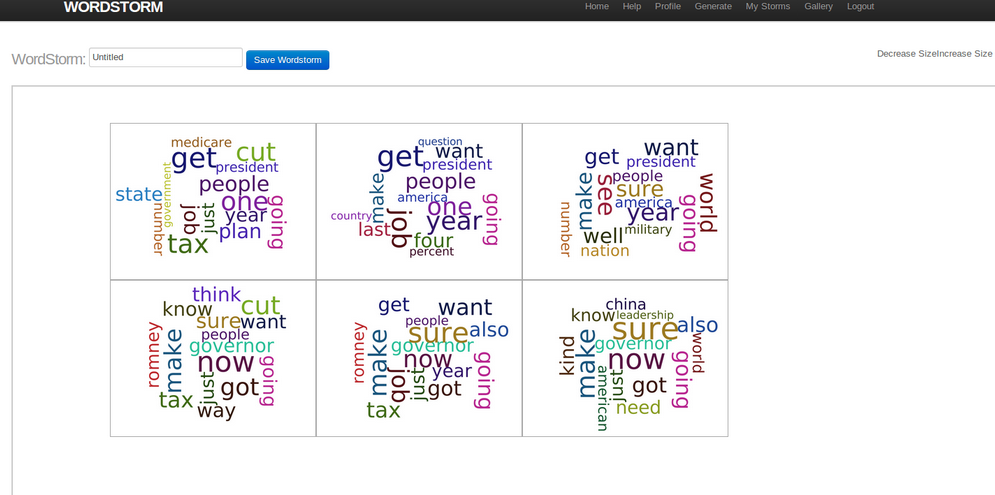
\includegraphics[width=0.7\textwidth]{MoveWord1.png}
  \caption{Initial configuration of the storm's clouds}
  \label{MoveWord1}

\end{figure}

\begin{figure}[!ht]
  \centering
  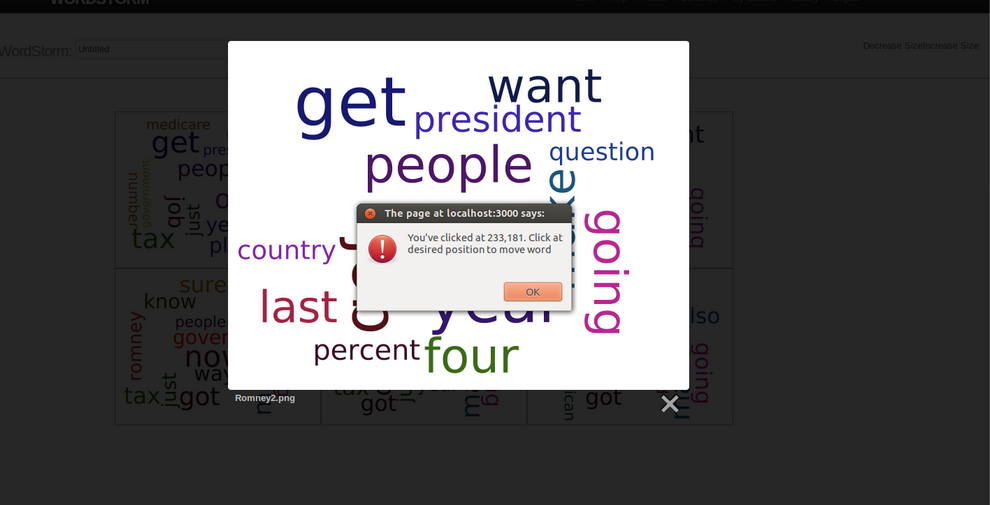
\includegraphics[width=0.7\textwidth]{MoveWord21.png}
  \caption{The move word interface, indicating that clicking again will move the word}
  \label{MoveWord2}

\end{figure}

\begin{figure}[!ht]
  \centering
  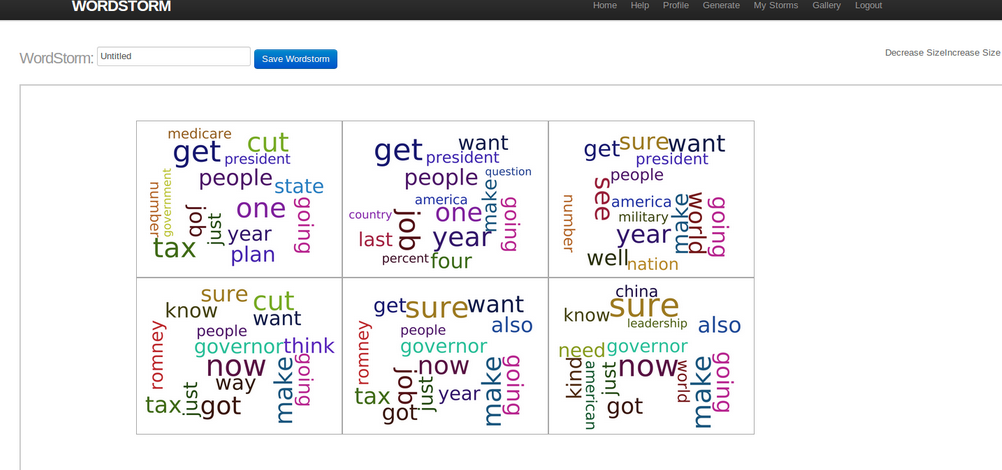
\includegraphics[width=0.7\textwidth]{MoveWord2.png}
  \caption{The word 'sure' has been selected and moved to the top middle from the center}
  \label{MoveWord3}

\end{figure}

\begin{figure}[!ht]
  \centering
  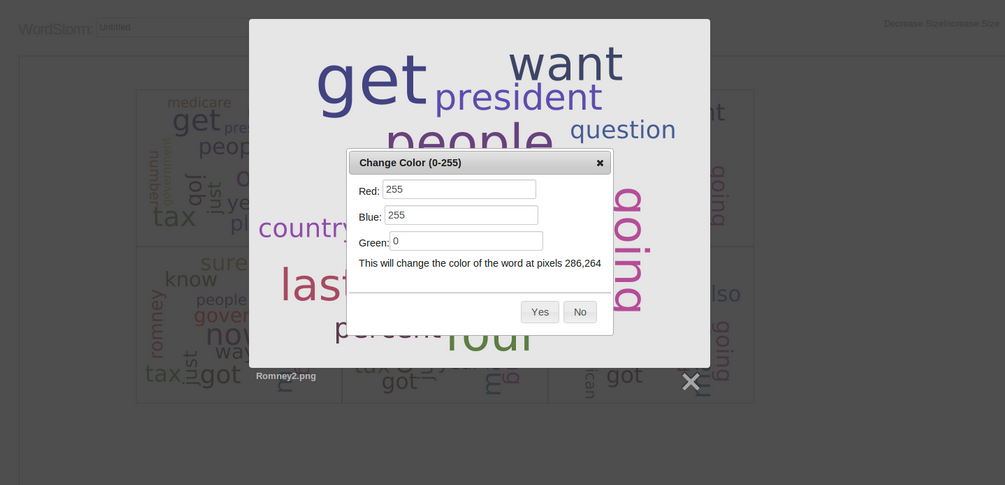
\includegraphics[width=0.7\textwidth]{MoveWord3.png}
  \caption{The color word interface, indicating that the information}
  \label{MoveWord4}

\end{figure}

\begin{figure}[!ht]
  \centering
  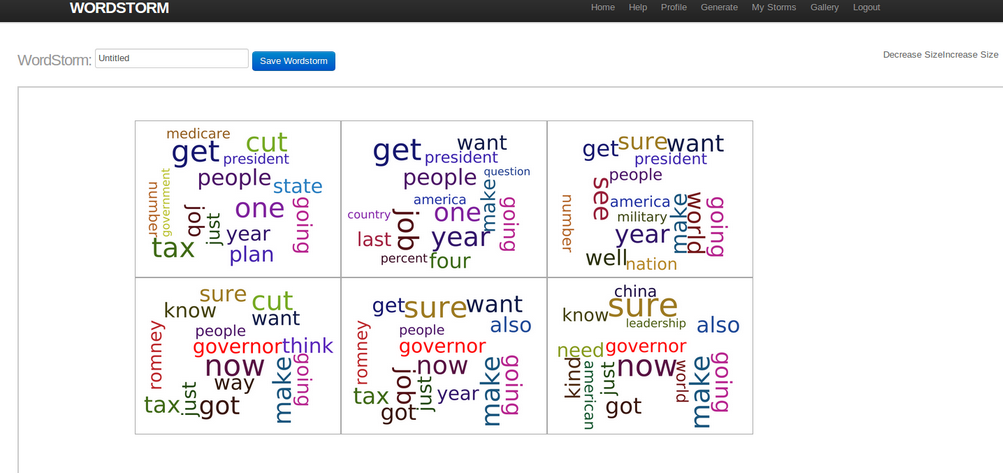
\includegraphics[width=0.7\textwidth]{MoveWord4.png}
  \caption{The word 'governor' has been recolored to red}
  \label{MoveWord5}

\end{figure}

\end{document}
